% !TEX program = lualatex

\documentclass[8pt,a4paper]{extarticle}
\usepackage[utf8]{inputenc}
\usepackage[british]{babel}
\usepackage[landscape, margin=1cm, bmargin=0.5cm, includefoot, footskip=0.5cm]{geometry}
\usepackage[textsize=tiny]{todonotes}
\usepackage{enumitem}
\usepackage{mdframed}
\usepackage{mathtools}
\usepackage{amsthm}
\usepackage{amssymb}
\usepackage{multicol,multirow}
\usepackage{subfiles}
\usepackage{tabularx}
\usepackage{bm}
\usepackage{xcolor}
\usepackage{graphicx}
\usepackage{accents}
\usepackage{pgfplots}
\usepackage{fancyhdr}
\usepackage[hidelinks]{hyperref}
\usepackage{nicefrac}

\newcommand{\cs}{Cheat sheet}
\newcommand{\csof}{Cheat sheet of }
\newcommand{\csAuthorName}{Carlos Lezama}
\newcommand{\csClass}{ }
\newcommand{\csClassCode}{ }
\newcommand{\csKeywords}{ }
\newcommand{\csTerm}{ }
\newcommand{\csSchool}{ITAM}

\pagestyle{fancy}
\renewcommand{\headrulewidth}{0pt}
\rhead{} 
\lhead{} 
\chead{} 
\cfoot{\csClass\ $\cdot$ \cs}
\lfoot{\csAuthorName}
\rfoot{Page \thepage}

\graphicspath{{./figures/}}

\usetikzlibrary{decorations.markings}
\pgfplotsset{compat=1.11}

\newmdtheoremenv [
	topline    = false,
	bottomline = false,
	leftline   = true,
	rightline  = false,
	linewidth  = 2.5pt,
	linecolor  = red!50
]{boxdef}{Definition}[section]

\mdtheorem [
	topline    = false,
	bottomline = false,
	leftline   = true,
	rightline  = false,
	linewidth  = 2.5pt,
	linecolor  = blue!40
]{boxtheo}{Theorem}[section]

\mdtheorem [
	topline    = false,
	bottomline = false,
	leftline   = true,
	rightline  = false,
	linewidth  = 2.5pt,
	linecolor  = black!20
]{boxprop}{Proposition}[section]

\mdtheorem [
	topline    = false,
	bottomline = false,
	leftline   = true,
	rightline  = false,
	linewidth  = 2.5pt,
	linecolor  = blue!40
]{boxlemma}{Lemma}[section]

\mdtheorem [
	topline    = false,
	bottomline = false,
	leftline   = true,
	rightline  = false,
	linewidth  = 2.5pt,
	linecolor  = blue!40
]{boxcor}{Corollary}[section]

\mdtheorem [
	topline    = false,
	bottomline = false,
	leftline   = true,
	rightline  = false,
	linewidth  = 2.5pt,
	linecolor  = black!20
]{boxrmk}{Remark}[section]

\newlist{numberlist}{enumerate}{1}
\setlist[numberlist, 1]{label={\arabic*.}, itemsep=0em, leftmargin=*,labelindent=0.5em}

\newlist{eqlist}{enumerate}{1}
\setlist[eqlist, 1]{label={\normalfont (\roman*)},itemsep=-0.2em, leftmargin=*,labelindent=-0.5em}

\newlist{bulletlist}{itemize}{1}
\setlist[bulletlist, 1]{itemsep=0em, leftmargin=0.5em, label={·}}

\setlength{\parindent}{0em}

\newenvironment{Figure}
  {\par\medskip\noindent\minipage{\linewidth}}
  {\endminipage\par\medskip}

\newcommand\tab[1][0.5em]{\hspace*{#1}}

\newcommand{\sectionbreak}{\vfill\ \columnbreak}

\usepackage{array}
\newcolumntype{P}[1]{>{\centering\arraybackslash}p{#1}}
\newcolumntype{M}[1]{>{\centering\arraybackslash}m{#1}}

% Economics
\newcommand{\E}{\resizebox{0.2cm}{!}{$\varepsilon$}}
\newcommand{\EE}{\mathcal{E}}
\newcommand{\I}{\mathcal{I}}
\newcommand{\LL}{\mathcal{L}}
\newcommand{\F}{\mathcal{F}}
\newcommand{\MRS}{\text{\normalfont MRS}}

% Statistics

% Mathematics
\DeclareMathOperator*{\argmin}{\arg \min}
\DeclareMathOperator*{\argmax}{\arg \max}
\newcommand{\deq}{\stackrel{\text{\normalfont def}}{=}}
\newcommand{\ie}{\text{\normalfont i.e.}}
\newcommand{\sgn}{\text{\normalfont sgn}}



% Class info
\renewcommand{\csClass}{Economics 4}
\renewcommand{\csClassCode}{ECO - 21104}
\renewcommand{\csTerm}{Spring 2021}
\renewcommand{\csKeywords}{ }

% PDF Metadata
\hypersetup{
    pdftitle={\csof \csClass},      
    pdfsubject={\csClass},
    pdfauthor={\csAuthorName},  
    pdfkeywords={}              
}

% Begin document
\begin{document}

\begin{titlepage}
    \begin{center}
	\vspace*{1cm}
	\Huge
        \textbf{\csClass}
	\vspace{0.5cm} \\
	\Large
        \cs\ $\cdot$ \csTerm
        \vfill
        \csAuthorName
	\vspace{0.8cm}
        \csClassCode\\
        \csSchool     
    \end{center}
\end{titlepage}

\begin{multicols}{3}
\setcounter{page}{1}

\section{General Equilibrium}

\subsection{Pure Exchange Economies}

\subsubsection*{Initial Assumptions}

\begin{bulletlist}
\item There are $m$ consumers such that $\I = \{1, \ldots, m\}$.
\item There are $n$ goods such that $\LL = \{1, \ldots, n\}$.
\item The preferences of each consumer are given by a utility function $u_i : \mathbb{R}^\LL \to \mathbb{R}$.
\item Each consumer can consume goods in $x_i \in \mathbb{R}_+^\LL$.
\item Each consumer has an initial endowment of $\omega_i \in \mathbb{R}_+^\LL$.
\item The ordered pair $(u_i, \omega_i)$ describes each consumer.
\item The utility functions represent neoclassical preferences.
\end{bulletlist}

\begin{boxprop}
	If $x \succ_i y$, then $u_i(x) > u_i(y)$.
\end{boxprop}

\begin{boxdef}[Exchange Economy]
	A \textbf{pure exchange economy} is: $$\EE = \left\langle \I, (u_i, \omega_i)_{i \in \I} \right\rangle,$$  where $\I$ is the set of agents; $u_i$ and $\omega_i$ are the utility function and initial endowment of the i-th consumer, respectively.
\end{boxdef}

\begin{boxdef}[Total Endowment]
	\[
		\Omega = \sum_{i \in \I} \omega_i
	.\] 
\end{boxdef}

\begin{boxdef}[Resource Allocation]
	The \textbf{resource allocation} is denoted by $X = (x_1, x_2, \ldots, x_m)$, where $\displaystyle x_i \in \mathbb{R}_{+}^{\LL}$.
\end{boxdef}

\begin{boxdef}[Feasible Allocation]
	The \textbf{feasible allocation} $\F$ of an economy $\EE$ is defined by:
	\[
		\F = \left\{ X = (x_1, x_2, \ldots, x_m)\ :\ x_i \in \mathbb{R}_{+}^{\LL},\ \sum_{i \in \I} x_i = \sum_{i \in \I} w_i \right\}
	.\] 
\end{boxdef}

\begin{boxdef}[Pareto-Efficiency]
	Let $\EE$ be an exchange economy. A \emph{feasible allocation of resources} $X = (x_1, x_2, \ldots, x_m)$ is said to be \textbf{Pareto-efficient} if and only if there is no other feasible allocation $\hat{X} = (\hat{x}_1, \hat{x}_2, \ldots, \hat{x}_m)$ such that, for every agent in $\I$, $u_i(\hat{x}_i) \ge u_i(x_i)$ and, for at least one agent $j$, $u_{j} (\hat{x}_{j}) > u_{j} (x_{j})$.
\end{boxdef}

\begin{boxdef}[Pareto-Dominance]
	Let $X$ and $\hat{X}$ be two feasible allocations. We say that $\hat{X}$ \textbf{Pareto-dominates} $X$ if and only if:
	\[
		u_i (\hat{x}_{i, 1}, \ldots, \hat{x}_{i, n}) \ge u_i (x_{i, 1}, \ldots, x_{i, n}), \quad \forall i \in \I
	,\]
	and there is at least one consumer $j$ such that:
	\[
		u_j (\hat{x}_{j, 1}, \ldots, \hat{x}_{j, n}) > u_j (x_{j, 1}, \ldots, x_{j, n})
	.\] 
\end{boxdef}

\begin{boxdef}[Contract Curve]
	The set of all \emph{Pareto-allocations} is known as the \textbf{contract curve}.
\end{boxdef}

\subsubsection*{Edgeworth Box}

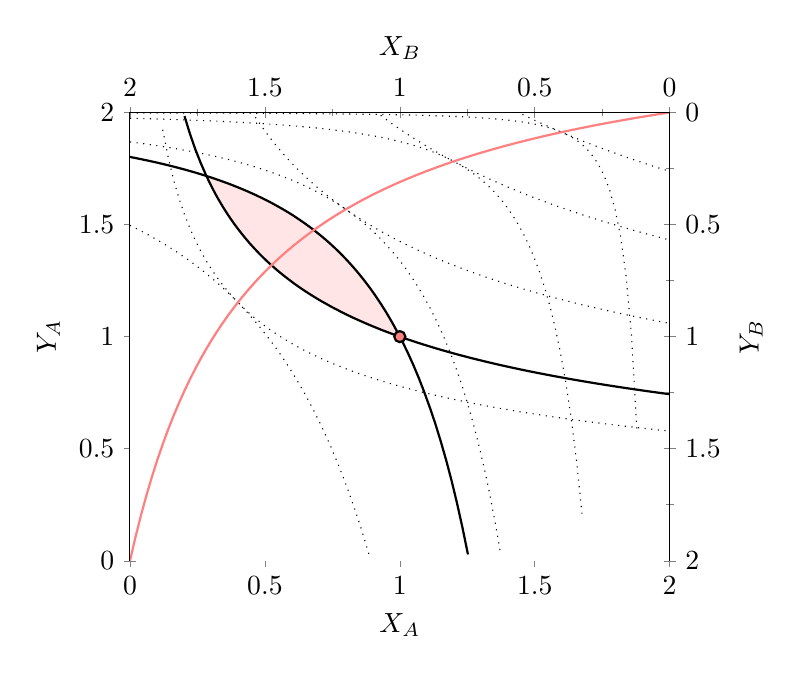
\begin{tikzpicture}[scale=1,thick]
  \def\alpha{0.7}
  \def\beta{0.3}
  \def\L{2}
  \def\K{2}
  \def\PK{0.5}
  \def\PL{0.5}
 
  \def\InitYA{((\PL*\L)^(1-\alpha))*((\PK*\K)^(\alpha))}		
  \def\InitYB{(((1-\PL)*\L)^(1-\beta))*(((1-\PK)*\K)^(\beta))}
 
  \def\La{0.2*\L}
  \def\Lb{0.4*\L}
  \def\Lc{0.6*\L}
  \def\Ld{0.8*\L}
 
  \def\Ka{
    \alpha*(1-\beta)*\K*\La/((1-\alpha)*\beta*(\L-\La)+\alpha*(1-\beta)*\La)}
  \def\Kb{
    \alpha*(1-\beta)*\K*\Lb/((1-\alpha)*\beta*(\L-\Lb)+\alpha*(1-\beta)*\Lb)}
  \def\Kc{
    \alpha*(1-\beta)*\K*\Lc/((1-\alpha)*\beta*(\L-\Lc)+\alpha*(1-\beta)*\Lc)}
  \def\Kd{
    \alpha*(1-\beta)*\K*\Ld/((1-\alpha)*\beta*(\L-\Ld)+\alpha*(1-\beta)*\Ld)}
 
  \def\YAa{((\La)^(1-\alpha)*((\Ka)^\alpha)}
  \def\YAb{((\Lb)^(1-\alpha)*((\Kb)^\alpha)}
  \def\YAc{((\Lc)^(1-\alpha)*((\Kc)^\alpha)}
  \def\YAd{((\Ld)^(1-\alpha)*((\Kd)^\alpha)}
 
  \def\YBa{((\L-\La)^(1-\beta)*((\K-\Ka)^\beta)}
  \def\YBb{((\L-\Lb)^(1-\beta)*((\K-\Kb)^\beta)}
  \def\YBc{((\L-\Lc)^(1-\beta)*((\K-\Kc)^\beta)}
  \def\YBd{((\L-\Ld)^(1-\beta)*((\K-\Kd)^\beta)}
 
  \begin{axis}[
      restrict y to domain=0:\K,
      samples = 100,     		
      xmin = 0, xmax = \L,
      ymin = 0, ymax = \K,
      xlabel = $X_A$,
      ylabel = $Y_A$,
      axis y line = left,    
      axis x line = bottom,
      y axis line style = {-}, 
      x axis line style = {-}
    ]
    \def\LineA{(\InitYA/\x^(1-\alpha))^(1/\alpha))};
    \def\LineB {\K-(\InitYB/(\L-\x)^(1-\beta))^(1/\beta)};
 
    \addplot [fill=red!20, opacity=0.5, draw=none,domain=0:\L] {\LineB}
      \closedcycle;
    \addplot [fill=white, draw=none,domain=0:\L] {\LineA} |- (axis cs:0,0)
      -- (axis cs:0,\K)--cycle; 
 
    \addplot[thin, dotted, mark=none, domain=0:\L]
      {(\YAa/\x^(1-\alpha))^(1/\alpha)};
    \addplot[thin, dotted, mark=none, domain=0:\L]
      {(\YAb/\x^(1-\alpha))^(1/\alpha)};
    \addplot[thick, mark=none, domain=0:\L] {(\LineA};
    \addplot[thin, dotted, mark=none, domain=0:\L]
      {(\YAc/\x^(1-\alpha))^(1/\alpha)};
    \addplot[thin, dotted, mark=none, domain=0:\L]
      {(\YAd/\x^(1-\alpha))^(1/\alpha)};
 
    \addplot[thin, dotted, mark=none, domain=0:\L]
      {\K-(\YBa/(\L-\x)^(1-\beta))^(1/\beta)};
    \addplot[thin, dotted, mark=none, domain=0:\L]
      {\K-(\YBb/(\L-\x)^(1-\beta))^(1/\beta)};
    \addplot[thick, mark=none, domain=0:\L] {\LineB};
    \addplot[thin, dotted, mark=none, domain=0:\L]
      {\K-(\YBc/(\L-\x)^(1-\beta))^(1/\beta)};
    \addplot[thin, dotted, mark=none, domain=0:\L]
      {\K-(\YBd/(\L-\x)^(1-\beta))^(1/\beta)};   
 
    \addplot[mark=none, domain=0:\L, color=red!50,thick]
      {\alpha*(1-\beta)*\K*\x/((1-\alpha)*\beta*(\L-\x)+\alpha*(1-\beta)*\x)};
    \addplot[thick, mark=*, fill=red!50] coordinates {(\L*\PL,\K*\PK)};    
  \end{axis}
 
  \begin{axis}[
      restrict y to domain = 0:\K,
      minor tick num = 1,
      xlabel = $X_B$,
      ylabel = $Y_B$,
      xmin = 0, xmax = \L,
      ymin = 0, ymax = \K,
      axis y line = right,
      axis x line = top,
      x dir = reverse,
      y dir = reverse,
      y axis line style = {-},
      x axis line style = {-}
    ]
  \end{axis}  
\end{tikzpicture}

\subsubsection*{General Case}

\begin{equation*}
\begin{aligned}
	\max_{\{ (x_{1, 1}, \ldots, x_{1, n}), \ldots, (x_{m, 1}, \ldots, x_{m, n})  \}}\ & u_1 (x_{1, 1}, \ldots, x_{1, n}) \\
	\text{subject to} \quad &  u_2 (x_{2, 1}, \ldots, x_{2, n}) \ge \bar{u}_2 \\
						    & \quad \vdots \\
							&  u_m (x_{m, 1}, \ldots, x_{m, n}) \ge \bar{u}_m \\
							& \sum_{i \in \I} x_{i, 1} \le \omega_1 \\
							& \quad \vdots \\
							& \sum_{i \in \I} x_{i, n} \le \omega_n
\end{aligned}
\end{equation*}

\begin{boxtheo}
	Let all utility functions be strictly increasing and quasi-concave, and	$((\hat{x}_{1,1}, \ldots, \hat{x}_{1, n}), \ldots, (\hat{x}_{m, 1}, \ldots, \hat{x}_{m, n}))$ be a feasible interior allocation. Then $((\hat{x}_{1,1}, \ldots, \hat{x}_{1, n}), \ldots, (\hat{x}_{m, 1}, \ldots, \hat{x}_{m, n}))$ is \textbf{Pareto-efficient} if and only if $((\hat{x}_{1,1}, \ldots, \hat{x}_{1, n}), \ldots, (\hat{x}_{m, 1}, \ldots, \hat{x}_{m, n}))$ exhausts all resources and, for all pairs of goods $\ell$, $\ell'$:
	\[
		\MRS(\ell, \ell') (\hat{x}_{1,1}, \ldots, \hat{x}_{1, n}) = \cdots = \MRS(\ell, \ell') (\hat{x}_{m,1}, \ldots, \hat{x}_{m, n})
	.\] 
\end{boxtheo}

\subsection{Competitive Equilibrium}

\subsubsection*{Initial Assumptions}

\begin{bulletlist}
\item There is a market for each good.
\item Every agent can access the market without any cost.
\item There is a unique price for each good and all consumers know the price.
\item Each consumer can sell her initial endowment in the market and use the income to buy goods and services.
\item Consumers seek to maximize their utility given their budget restriction, independently of what everyone else is doing.
\item There is no centralized mechanism.
\item People may not know others preferences or endowments.
\item There is perfect competition (i.e. everyone is a price-taker).
\item The only source of information agents are prices.
\end{bulletlist}

\begin{boxdef}[Competitive Equilibrium]
	An ordered pair of an allocation and a price vector, $(x^*, p = (p_1, \ldots, p_n))$, is called a \textbf{competitive equilibrium} if the following conditions hold:
	\begin{eqlist}
	\item $\forall i \in \I,\ x^*_i = (x^*_{i, 1}, \ldots, x^*_{i, n})$ solves the following maximization problem: 
		\begin{equation*}
		\begin{aligned}
			\max_{\{x_i\}}\	  & u_i(x_i) \\
			\text{\normalfont subject to} \quad & wh + p \cdot x_i \le p \cdot \omega_i = \sum_{\ell \in \LL} p_\ell \omega_{i, \ell}.
		\end{aligned}
		\end{equation*}
	\item Markets clear, i.e. $\displaystyle \sum_{i \in \I} x^*_{i, \ell} = \sum_{i \in \I} \omega_{i, \ell},\ \forall \ell \in \LL$.
	\end{eqlist}
\end{boxdef}

\begin{boxprop}
	Given, at least, one consumer with strictly monotone preferences. Then, if $(x^*, p)$ is a competitive equilibrium, $p_1, p_2, \ldots, p_n > 0$.
\end{boxprop}

\newpage

\begin{boxprop}
	Given, at least, one consumer with weakly monotone preferences. Then, if $(x^*, p)$ is a competitive equilibrium, for at least one $\ell$, $p_\ell > 0$.
\end{boxprop}

\begin{boxprop}
	Let $(x^*, p)$ be a competitive equilibrium. Then, $(x^*, cp)$ is also a competitive equilibrium, $\forall c \in \mathbb{R}_+$.
\end{boxprop}

\begin{boxtheo}[Walras' Law]
	If the consumer $i$ has weakly monotone preferences and also $\hat{x}_i \in x^*_i (p)$, then:
	\[
		p \cdot \hat{x}_i = \sum_{\ell \in \LL} p_\ell \hat{x}_{i, \ell} = \sum_{\ell \in \LL} p_\ell \omega_{i, \ell} = p \cdot \omega_i
	.\] 
\end{boxtheo}

\begin{boxcor}[Walras' Law]
	Given weakly monotonic utility functions and $p = (p_1, \ldots, p_n)$ such that $p_n > 0$. If any $(x^*, p)$ in which maximization condition holds, $\forall i \in \I$, and markets clear $\forall \ell = 1, 2, \ldots, n - 1$; then, the market clearing condition holds for commodity $n$ as well.
\end{boxcor}

\begin{boxtheo}[Fixed Point]
	For any continuous function $f : \triangle^{n - 1} \to \triangle^{n - 1}$, there exists a point $p^* = (p^*_1, p^*_2, \ldots, p^*_n)$ such that $f(p^*) = p^*$, where $\displaystyle \triangle^{n - 1} = \left\{(p_1, p_2, \ldots, p_n) \in \mathbb{R}_+^\LL : \sum_{\ell \in \LL} p_\ell = 1 \right\}$.
\end{boxtheo}

\begin{boxdef}[Shortage]
	We define \textbf{shortage} or \textbf{excess demand} as follows:
	\[
		Z(p) = (z_1(p), z_2(p), \ldots, z_n(p)) = \sum_{i \in \I} x^*_i(p) - \sum_{i \in \I} \omega_i
	.\] 
\end{boxdef}

\begin{boxprop}
	$p$ is a competitive equilibrium if and only if $Z(p) = 0$.
\end{boxprop}

\subsubsection*{Excess Demand Properties}

\begin{eqlist}
\item Continuous in $p$.
\item Homogeneous of degree zero.
\item $p \cdot Z(p) = 0$.
\end{eqlist}

\begin{boxprop}
	The equilibrium is not unique.
\end{boxprop}

\begin{boxtheo}[Welfare I]
	Given any pure exchange economy such that all consumers have weakly monotonic utility functions. Then, if $(x^*, p)$ is a competitive equilibrium, $x^*$ is a Pareto-efficient allocation.
\end{boxtheo}

\begin{boxtheo}[Welfare II]
	Given an economy $\displaystyle \EE = \left\langle \I, (u_i, w_i)_{i \in \I} \right\rangle$ where all consumers have weakly monotonic, quasi-concave utility functions. If $(x_1, x_2, \ldots, x_m)$ is a Pareto-optimal allocation; then, there exists a redistribution of resources $(\hat{w}_1, \hat{w}_2, \ldots, \hat{w}_m)$ and some prices $p = (p_1, p_2, \ldots, p_n)$ such that:
	\begin{eqlist}
	\item $\displaystyle \sum_{i \in \I} \hat{w}_i = \sum_{i \in \I} w_i$.
	\item $(p, (x_1, x_2, \ldots, x_m))$ is a competitive equilibrium of the economy $\EE$.
	\end{eqlist}
\end{boxtheo}

\newpage

\section{Monopoly and Monopsony}

\newpage

\section{Game Theory}

\vfill\eject
\columnbreak
\end{multicols}
\end{document}
